\documentclass[12pt,uplatex]{jsarticle}   % 日本語
\usepackage{tcu-thesis}
\usepackage{fancyhdr}
\usepackage{bm} % 太字の数式
\usepackage{amssymb} % 数式
\usepackage{amsmath} % 数式
\usepackage{float} % 図表の位置
\usepackage{listings} % ソースコード
\usepackage{color} % ソースコードの色付け

% ソースコードのスタイル設定
\lstset{
  basicstyle=\ttfamily\footnotesize,
  numbers=left,
  numberstyle=\tiny\color{gray},
  stepnumber=1,
  numbersep=5pt,
  backgroundcolor=\color{white},
  showspaces=false,
  showstringspaces=false,
  showtabs=false,
  frame=single,
  rulecolor=\color{black},
  tabsize=2,
  captionpos=b,
  breaklines=true,
  breakatwhitespace=false,
  title=\lstname,
  keywordstyle=\color{blue},
  commentstyle=\color{green},
  stringstyle=\color{red},
  escapeinside={\%*}{*)},
  morekeywords={*,...}
}

% Python用のスタイル設定
\lstdefinestyle{python}{
  language=Python,
  keywordstyle=\color{blue},
  commentstyle=\color[RGB]{0,100,0},     %DarkGreen
  stringstyle=\color[RGB]{128,0,0},      %Maroon
  frame=single,
  breaklines=true,
  basicstyle=\ttfamily\footnotesize
}

% Jupyter Notebook用のスタイル設定
\lstdefinestyle{jupyter}{
  language=Python,
  keywordstyle=\color{blue},
  commentstyle=\color[RGB]{0,100,0},     %DarkGreen
  stringstyle=\color[RGB]{128,0,0},      %Maroon
  frame=single,
  breaklines=true,
  basicstyle=\ttfamily\footnotesize,
  morekeywords={In, Out, print}
}


% アルゴリズムのレイアウト
\newenvironment{algorithm_step}
{\begin{list}{}
    {\setlength{\leftmargin}{6em}  % Step X)の部分の幅
     \setlength{\itemindent}{0em}
     \setlength{\labelsep}{0em}
     \setlength{\labelwidth}{6em}  % Step X)の部分の幅
     \setlength{\itemsep}{1em}     % ステップ間の縦方向の間隔
     \renewcommand{\makelabel}[1]{##1\hfill}}}
{\end{list}}

% 数式カウンターの定義
\newcounter{myeqcounter} % 独自カウンターを定義

\newcommand{\autoequation}[1]{
\refstepcounter{myeqcounter} % カウンターを進める
\begin{equation}
#1 \tag{\themyeqcounter} % カウンター値をタグに適用
\end{equation}
}


% オリジナルマクロ by Kyohei Fushida and Kenji Fujiwara
\newcommand{\li}{\item}
\newcommand{\ol}[1]{\begin{enumerate}#1\end{enumerate}}
\newcommand{\ul}[1]{\begin{itemize}#1\end{itemize}}
\newcommand{\dl}[1]{\begin{description}#1\end{description}}
\newcommand{\equ}[1]{\begin{equation}#1\end{equation}}
\newcommand{\eqenum}[1]{\begin{align}#1\end{align}}
\newcommand{\eqa}[1]{\begin{align}#1\end{align}}
\newcommand{\eqmul}[1]{\begin{equation}\begin{split}#1\end{split}\end{equation}}
\usepackage{xcolor}

%\newcommand{\figref}[1]{図\ref{#1}}
%\newcommand{\tabref}[1]{表\ref{#1}}
\renewcommand{\subsecref}[1]{\ref{#1}項}
\newcommand{\chapref}[1]{\ref{#1}章}

\definecolor{darkgreen}{rgb}{0, 0.5, 0} %下の色指定で使う
\definecolor{whitesmoke}{rgb}{0.99, 0.99, 0.99} %下の色指定で使う
\newcommand{\red}{\color{red}}%red
\newcommand{\blue}{\color{blue}}
\newcommand{\green}{\color{teal}}
\newcommand{\purple}{\color{violet}}%violet
\newcommand{\black}{\color{black}}
\newcommand{\ea}{\xspace\emph{et al.}\xspace}
\newcommand{\TODO}[1]{\nb{TODO:}{#1}}


\newcommand{\methods}{\#methods}
\newcommand{\colorrow}{\rowcolor[rgb]{0.851,0.851,0.851}}
\newcommand{\colorcel}{\cellcolor[rgb]{0.851,0.851,0.851}}
\def\et{\xspace et\ al.\xspace}
\def\ie{i.e.,\xspace}
\def\eg{e.g.,\xspace}
\newcommand{\nb}[2]{
    \fcolorbox{gray}{yellow}{\bfseries\sffamily\scriptsize#1}
    {\sf\small\textit{\textcolor{blue}{#2}}}
   }

\newtheorem{defi}{定義}
\newtheorem{hypo}{仮説}

% 必要なパッケージの読み込み
% とりあえず最低限使っておいて欲しいパッケージのみ書いています.
% 色々なパッケージがあります.藤原が過去に使ってたパッケージなどは博士論文のファイルを参照してください.
\usepackage[dvipdfmx]{graphicx}
\usepackage{cite} % 参考文献を [3,4]のようにまとめるのに便利.
\usepackage{url} % urlを記載するときに使う.

% 参考文献を引用された順で出力する
\bibliographystyle{junsrt}

% 学籍番号
\studentnumber{2172010}

% 日本語題目
\title{入力データの構造を考慮したLowProFoolアルゴリズム\\による敵対的サンプルの生成に関する研究}

% 英語題目
\etitle{Generation of Adversarial Samples Using Modified LowProFool Algorithm with Consideration of Input Data Structure}

% 日本語氏名(姓と名の間に空白(半角)を入れて下さい)
\author{有馬 祥太}

% 欧文氏名(first name, last name の順に記入し,先頭文字のみを大文字にする.)
\eauthor{Shota Arima}

% 専攻
\department{\media}
\course{\jsys}

% 論文提出年月日
\syear{2025}
\smonth{1}
\sday{30}

% % キーワード5〜6個 (in LaTeX)
% \keywords{敵対的サンプル,表形式データ,LowProFoolアルゴリズム,データ離散化,特徴量重要度}

% % 5 or 6 Keywords (in LaTeX)
% \ekeywords{Adversarial Samples, Table Data, LowProFool Algorithm, Data discretization, Importance of Features}

% 内容梗概 (in LaTeX)
%   Abstractは必須です.
%   サンプルほど長々と書く必要はありません.
%   注: 行の先頭が\\で始まらないようにすること.
% \abstract{%
% この研究では,機械学習モデルに対する敵対的サンプル生成において,表形式データのおける敵対的サンプルの特性を考慮した改良手法を提案しています.
% 従来のLowProFoolアルゴリズムでは特定の特徴量に対して過度にノイズが付与されてしまう可能性と離散値を持つ表形式データに対して連続値の敵対的サンプルを生成してしまう課題がありました.
% そこで本研究では,特徴量の重要度算出方法を改善し,出力データの離散化を行うことで,より自然な敵対的サンプルの生成を実現しました.
% 実験結果から,提案手法により過度なノイズの付与を抑制でき,より現実的な敵対的サンプルの生成が可能になりました.
% }

%%%%%%%%%%%%%%%%%%%%%%%%% document starts here %%%%%%%%%%%%%%%%%%%%%%%%%%%%

\begin{document}
%
% 表紙 および アブストラクト
%

\begin{center}
    \vspace*{5cm} % 上部の余白調整

    {\Large 2024 年度 卒業論文} % 大きめのフォント
    \vspace{3cm}

    {\LARGE 入力データの構造を考慮した\\LowProFoolアルゴリズムによる\\敵対的サンプルの生成に関する研究} % タイトル
    \vspace{2cm}

    \begin{flushright}
        {\large 東京都市大学} \\
        {\large メディア情報学部情報システム学科} \\
        {\large 三川研究室} \\
        {\large 2172010 有馬 祥太} \\
        {\large 指導: 三川 健太 准教授} \\
    \end{flushright}

\end{center}

% \titlepage
% \jabstractpage
%
% 目次
%
\tableofcontents
\newpage

% 以降本文
\pagenumbering{arabic} % ページ番号をアラビア数字に戻す

% この章構成はあくまで一例です.
% \section:章
% \subsection: 節
% \subsubsection: 項
% として使ってください.
% 研究の内容によって自分が適切だと思う章構成を考えて下さい.
% もちろん構成について藤原と相談するのも良いと思います.
% \section{テンプレート}
% %サンプルです.必要なければファイルごと削除してください.
% 「はじめに」では研究の背景を述べつつ研究の目的を述べるのが一般的です.
% 仰々しい論文の場合は論文の構成(以降の章構成)を説明したりもします.

% 最初は世の中(といっても情報系分野ぐらいで十分ですが)全体の背景を述べつつ,
% 徐々に的を絞ってどうして自身の研究を行う必要があるのかを上手く説明できると素晴らしいです.
% 研究の背景となる課題や既存研究を紹介する際には必ず参考文献を引用するようにしましょう.

% 「はじめに」は他の章に比べて非常に作成が難しいです.
% どういう流れで書けばいいのか困った際は指導教員に聞くのもよいと思いまし,とりあえず書ける章(自分が実際に手を動かした章)から書いていくのも良いと思います.


% \subsection{論文を書く際の注意事項}
% \begin{itemize}
%     \item 句読点は全角のカンマとピリオドである「,」と「.」を使って下さい.卒論執筆期間中は一時的にIMEの設定を変更して常にカンマとピリオドが使用されるようにしておくと安全だと思います.
%     \item 表記揺れに注意しましょう.
%     \item ですます調はNGです.
%     \item 未定義語は使わない.一般的でない用語が出てくるタイミングで必ず説明を入れる.
% \end{itemize}


\section{序論}
\subsection{研究背景}
近年,情報技術の進歩に伴い,機械学習モデルが多くの分野で活用され始めている.金融,医療,交通などの領域において,膨大なデータを解析することで効率的かつ高度な意思決定が可能となり,私たちの生活は利便性と効率性を向上させる多くの恩恵を受けられるようになった.一方で,これらの機械学習モデルに依存する場面が増えるにつれて,機械学習モデルの誤作動や悪用が引き起こすリスクも拡大している。例えば,ば,医療分野における誤診や,交通分野における自動運転車の誤作動が発生した場合,人的被害や社会的混乱を招く可能性がある.そのため、機械学習モデルがもたらす利便性を最大化しつつ、それらが安全かつ信頼できるものであることを保証することが極めて重要である.こうした状況の中で特に注目されている課題が、機械学習モデルの脆弱性を悪用した攻撃手法である。その一例として、敵対的サンプルによる攻撃が挙げられる。敵対的サンプルとは,人間には見分けのつかない微細なノイズをデータに付与することで機械学習モデルの誤分類を引き起こすデータである.このようなデータを用いた攻撃によって機械学習モデルが重大な誤りを犯す可能性がある.例えば,銀行のローンの審査システムについての機械学習モデルを想定すると,本来なら認可すべきではないリスクの高いローンを誤って承認されるケースが考えられる.このような問題に対処するため,機械学習モデルの安全性が求められており,よりノイズの小さい敵対的サンプルの生成によってよりロバストな機械学習モデルの構築の貢献し,安全性を向上に寄与すると考えられる.

敵対的サンプルは主に画像データを対象に研究が行われてきた.特に自動運転における物体検知の研究においてこの敵対的サンプルによる誤分類問題がよく取り上げられていた.しかし画像データだけではなく,表形式データに対する攻撃もまた無視できない課題である.表形式データは,金融,医療,ビジネス領域で広く利用されており,機械学習モデルの入力データとしても多く用いられている.画像用の敵対的サンプル生成手法を適用すると非現実的なサンプルが生成される可能性がある.そのため,表形式データの敵対的サンプルの生成手法では,入力データの特性に合わせた敵対的サンプルの生成手法が求められる.

\subsection{研究目的}
上記の議論のもと本研究では,表形式データの特徴を考慮したより自然な敵対的サンプルを生成する手法を提案することを目的とする.元データの分布に合わせてより少ないノイズを加え,連続値として出力される非現実的なサンプルの問題を解決する.以上より,より自然な表形式データに対する敵対的サンプルの生成が可能となる.提案手法により,本研究の目的が達成されることで,既存の機械学習モデルの弱点をより正確に把握することが可能となる.これにより,モデルの脆弱性を評価し,敵対的サンプルによる誤分類を防ぐための対応策を事前に講じることができ,モデルの安全性向上に貢献することができる.

\section{準備}
% \subsection{問題設定}
% 本研究では,銀行のローンの審査システムについての機械学習モデルを想定し,認可拒否について誤分類を引き起こす敵対的サンプルを生成することを考える.銀行のローンを申請する顧客情報と正解データをもとに機械学習モデルが学習し,テストデータに対する分類結果を出力する.敵対的サンプルによる誤分類は,銀行にとってリスクの高いローンを誤って認可してしまう可能性がある.このような問題に対処するため,機械学習モデルの安全性が求められており,敵対的サンプルに対する防御手法が必要である.また同時に,モデルの脆弱性を理解することは,安全性を向上させるために重要である.

\subsection{ニューラルネットワーク}
ニューラルネットワークは、機械学習の一種であり、多層のノード(ニューロン)から構成されるモデルですある。各ノードは入力を受け取り、重み付けされた和を計算し、活性化関数を通じて出力を生成する。ニューラルネットワークは、以下のような構造を持ちます。

\begin{figure}[H]
    \centering
    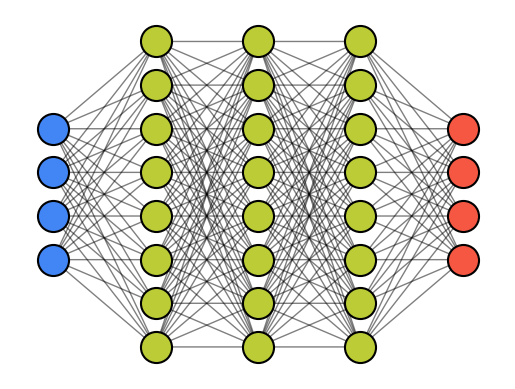
\includegraphics[width=0.8\textwidth]{images/struc_NN.png}
    \caption{ニューラルネットワークの構造}
    \label{fig:adversarial_learning1}
\end{figure}

\begin{itemize}
    \item 入力層: 青色のノードの部分であり、モデルに入力されるデータを受け取る層である。各ノードは特徴量を表す。
    \item 隠れ層: 黄色のノードの部分であり、入力層と出力層の間に位置する層で、複数の 層を持つことができる。各ノードは前の層の出力を入力として受け取り、重み付けされた和を計算し、活性化関数を通じて出力を生成する。
    \item 出力層: 赤色のノードの部分であり、モデルの最終的な予測を生成する層である。分類問題では、各ノードはクラスを表し、回帰問題では連続値を出力する。
\end{itemize}

活性化関数は、ニューラルネットワークの各ノードで計算される重み付けされた和に対して、非線形性を導入するために使用される。非線形性は、入力と出力が直接表現できないことを示しており、これによりモデルが複雑なパターンを学習できるようになる。\cite{book-deeplearning}

\subsection{敵対的学習}
\subsubsection{敵対的学習の概要}
機械学習モデルは,膨大なデータからパターンを学習し,予測や分類を行う.しかし,そのデータに微小な変更(敵対的サンプル)が加えられることで,人間には明らかに正しいと認識されるデータを,モデルが誤分類してしまうケースがある.これにより,安全性が求められる分野(例:顔認証や金融審査など)で深刻な問題が発生する可能性があります.

敵対的学習は,機械学習モデルの堅牢性を向上させるための手法として誕生した.従来の機械学習モデルは,訓練データに対して高い精度を示す一方で,敵対的サンプルと呼ばれる微細ななノイズを含むデータに対しては脆弱である.

goodfellowらの研究\cite{goodfellow2015explaining}でこの敵対的学習について提案された.この手法では,正常データと敵対的サンプルの特徴をAIに学習させる防御手法である.機械学習モデルの学習時において,正常データと敵対的サンプルに対する誤差(Loss)をそれぞれ計算する。以下の式(1)のように先ほどの誤差を足し合わせ、これらを基にモデルの重み $\bm{w}$ を更新し,敵対的サンプルの特徴を学習する.

\autoequation{\alpha \cdot Loss(x,y) + (1-\alpha) \cdot Loss(\tilde{x},y)}

ここで、$\alpha$ は元データと敵対的サンプルの誤差のバランスを調整するパラメータであり、$Loss(x,y)$ は元データ $x$ とラベル $y$ に対する誤差、$Loss(\tilde{x},y)$ は敵対的サンプル $\tilde{x}$ とラベル $y$ に対する誤差を表します。

\subsubsection{敵対的学習の流れ}
以下に実際の敵対的学習の流れを示す.\cite{MBSD-AdversarialTraining}

\begin{enumerate}

    \item 学習中の機械学習モデルを利用して敵対的サンプルを作成する

    下に示す図1は,敵対的学習の最初のステップである,元データから敵対的サンプルを作成するプロセスを示している.この図では,元画像に微細なノイズを加えることで,モデルが誤分類を引き起こす敵対的サンプルが生成される様子を視覚的に表している.最初に元データの画像を機械学習モデルに入力し,予測ラベル $y$ を得る.次に,この予測と正解データを比較した誤差を $Loss$ 関数で計算し,この誤差を最小化するように敵対的サンプルを生成している.
    
    \begin{figure}[H]
        \centering
        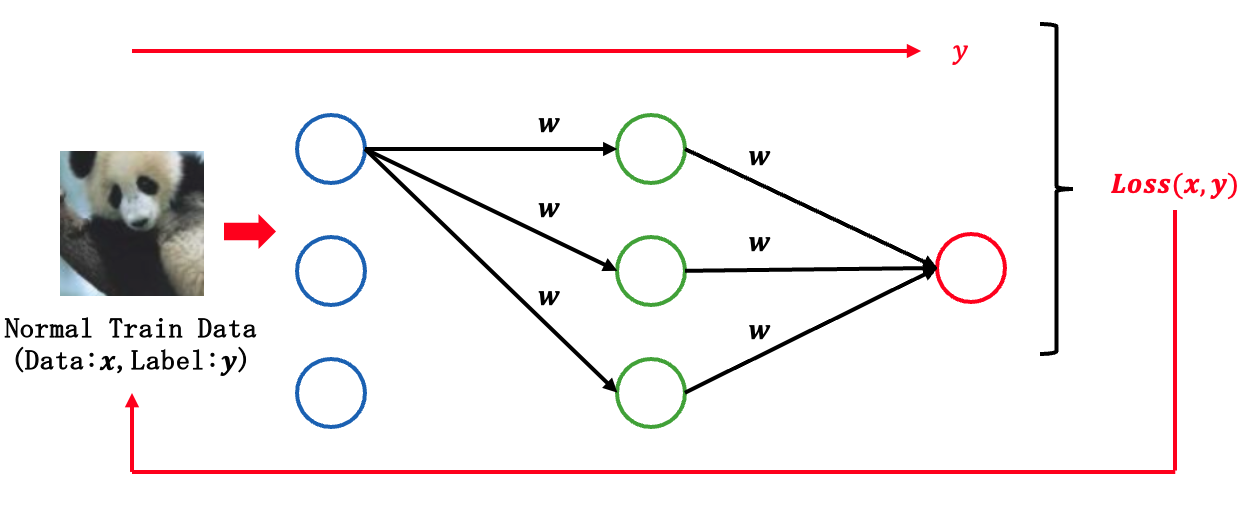
\includegraphics[width=0.8\textwidth]{images/敵対的学習1.png}
        \caption{敵対的学習1:敵対的サンプルを生成}
        \label{fig:adversarial_learning1}
    \end{figure}
    
    \item 機械モデルに正常なデータ $\bm{x}$ と敵対的サンプル $\bm{x}'$ を入力し,それぞれの誤差 $Loss$ を得る

    図2は,生成された敵対的サンプルと元データとの入力の違いを比較している.元データは,すべて純粋な特徴量から構成され,モデルが意図通りに分類などを行うための基盤となる.一方敵対的サンプルは,元データに対して微細なノイズを加えたもので,このノイズはほとんど人間には認識できないものである.しかしモデルの分類結果を大きく変えてしまうため入力の誤差を出力している.

    \begin{figure}[H]
        \centering
        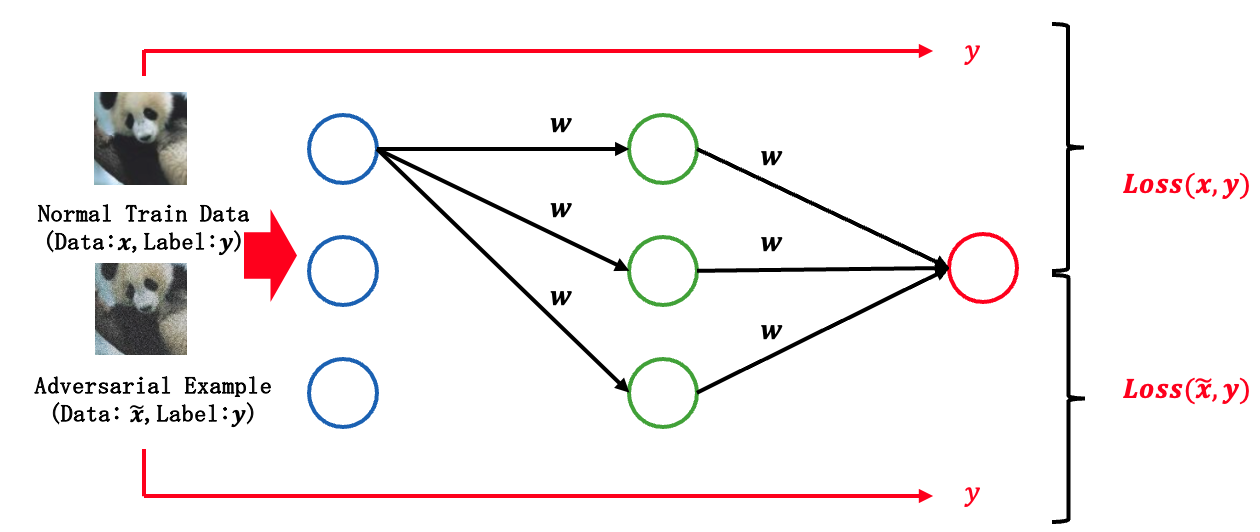
\includegraphics[width=0.8\textwidth]{images/敵対的学習2.png}
        \caption{敵対的学習2:元データと敵対敵サンプルの誤差の導出}
        \label{fig:adversarial_learning2}
    \end{figure}

    \item それぞれ得た誤差 $Loss(x, y), Loss(x', y)$ に重み係数 $\alpha$ をつけて足し合わせる

    図3では,元データによって生成された誤差と敵対的サンプルによって生成された誤差を取得し,足し合わせている.この誤差をどのようなバランスで機械学習モデルに組み込んでいくかという重要なステップである. 上記の式(1)にある誤差の足し合わせの式用いて行われる。
    
    \begin{figure}[H]
        \centering
        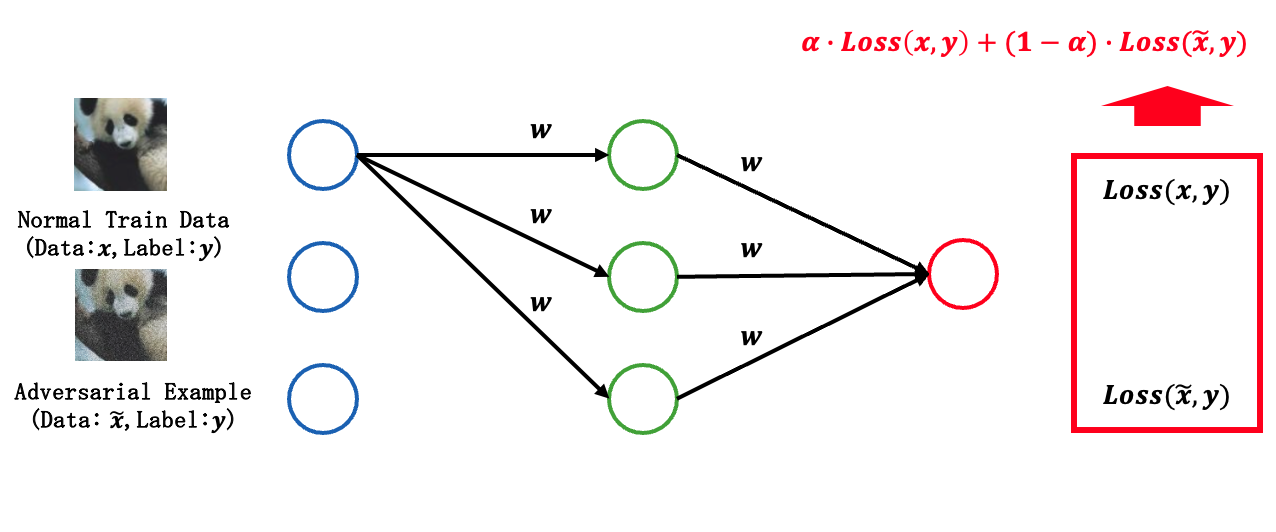
\includegraphics[width=0.8\textwidth]{images/敵対的学習3.png}
        \caption{敵対的学習3:元データと敵対敵サンプルの誤差の足し合わせ}
        \label{fig:adversarial_learning3}
    \end{figure}

    \item 足し合わされた誤差 $Loss$ が最小となるように,重み $\bm{w}$ を更新する

    図4では,先ほど生成された敵対的サンプルの誤差を含めた誤差を用いて,機械学習モデルの更新を行う.この作業は敵対的サンプルによる誤分類にも耐えられるような分類を行うために図1で学習された機械学習モデルの重み $w$ を敵対的サンプルに対応させるため更新する.
    先ほどの式(1)を最小化することで,重み $w$ を $w_{\_new}$ に更新する.これにより,敵対的サンプルの挙動を抑えることができた機械学習モデルを作成することができる.
    
    \begin{figure}[H]
        \centering
        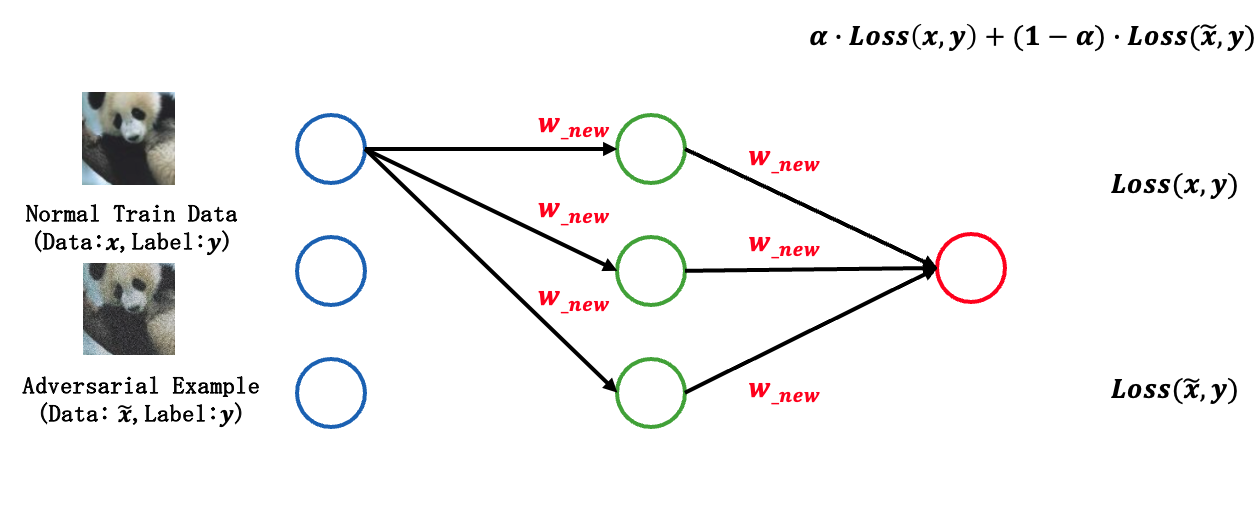
\includegraphics[width=0.8\textwidth]{images/敵対的学習4.png}
        \caption{敵対的学習4:重みの更新}
        \label{fig:adversarial_learning4}
    \end{figure}

\end{enumerate}

以上の流れにより,敵対的サンプルを学習過程の中に組み込むような敵対的学習を行うことで,機械学習モデルが敵対的サンプルの挙動に対応することができ,堅牢性を向上させることができる.

\subsection{敵対的サンプル}
敵対的学習を実現する上で中心となるのが,敵対的サンプルの生成である.ここでは,敵対的サンプルがどのようにモデルに影響を与えるかを詳しく説明する.
研究背景で触れたように敵対的サンプルとは,人間には見分けのつかない微細なノイズをデータに付与することで機械学習モデルの誤分類を引き起こすデータである.\cite{MBSD-AdversarialExample}運用している機械学習モデルを狙った攻撃に使用されることがある.

敵対的サンプルによる誤分類を確認した実験をGoodfellowらが行っている\cite{goodfellow2015explaining}.
\begin{figure}[H]
    \centering
    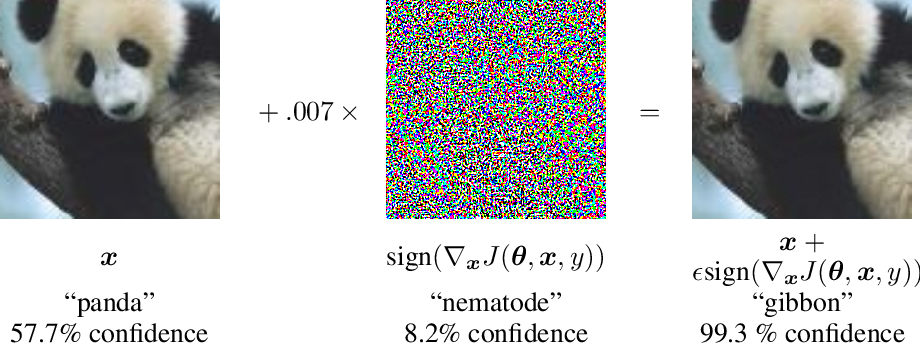
\includegraphics[width=0.8\textwidth]{images/goodfellow_panda.png}
    \caption{敵対的サンプルの例:パンダの敵対的サンプル画像をテナガザルと判断\cite{goodfellow2015explaining}}
    \label{fig:adversarial_example}
\end{figure}

図5は,敵対的サンプルの具体例として,パンダの画像に微細なノイズを加えた結果,モデルがテナガザルと誤分類した事例を示している.この例は,敵対的サンプルが人間にはほとんど判別できない変更であっても,モデルにとっては大きな影響を与えることを視覚的に示しています.

このように画像データに対する敵対的サンプルの生成は行うことができることがわかった.しかし,表形式データに対する敵対的サンプルは,先ほどの手法を用いて生成することは難しいという問題がある.その理由として,表形式データの特徴量は画像データと異なる性質を持つためである.画像データの場合,各ピクセルの値は0から255の範囲の連続値として扱うことができ,わずかな変化は人間の目では認識できないことが多い.一方で,表形式データの特徴量には,年齢や収入といった数値データだけでなく,性別や職業といったカテゴリカル変数も含まれる.また,各特徴量は独立した意味を持っており,それぞれの特徴量の変化は明確な意味の変化を伴う.例えば,先ほどのパンダの画像の場合,個々のピクセル値にわずかな変化を加えても,人間にとってはそれが「パンダの画像」であることに変わりはない.しかし,ローン申請データにおいて,年収を示す特徴量に対してわずかな変化を加えた場合,その変化は申請者の経済状況を直接的に変えてしまう可能性がある.さらに,職業などのカテゴリカルデータの場合,わずかな変化という概念自体が適用できない.このような表形式データの特性により,画像データに対する敵対的サンプル生成手法をそのまま適用することは適切ではない.そこで,表形式データの特性を考慮した新たな敵対的サンプル生成手法が必要となる.特に,各特徴量の重要度や,特徴量の種類(連続値かカテゴリカル値か)を考慮した手法が求められる.




\section{従来手法}
\subsection{LowProFool}
\subsubsection{概要}
表形式データに対する敵対的サンプルの生成手法として,Balletらが提案したLowProFool\cite{ballet2019imperceptible}がある.表形式データの特徴として識別に寄与する各特徴量の重要度が異なることが多い.LowProFoolはこの点に着目し各特徴量の重要度を元データから算出し,それに基づいたノイズを付加することで誤分類を引き起こし,検知されにくい敵対的サンプルを生成する.この手法は,深層学習モデルを用いて敵対的サンプルを用いて敵対的サンプルを生成する点に特徴がある.具体的には,ニューラルネットワークを用いて元データに対するノイズを最適化し,モデルの誤分類を誘発する.このアプローチにより,より高度な特徴抽出とノイズ付加が可能となり,従来の手法よりも効果的な敵対的サンプルを生成することができる.

\subsubsection{LowProFoolの問題設定}
LowProFoolは検知されにくい敵対的サンプルを生成するため,以下の最適化問題を解く.

まず、敵対的サンプルを生成するにあたっての元のデータを $\bm{x}$ とする。そしてこの元データにノイズを加えるノイズベクトル $\bm{r}$を定義する.また、各特徴量に対する重要度を $\bm{v}$ と表す.ノイズは $A$ で定められる現実的な値域をとるように制限される.元データによる分類ラベル $\bm{x}$ とすると,敵対的サンプル $\bm{\tilde{x}}$ は異なるラベル $t$ を持つ.

LowProFoolでは以下の最適化問題を解き敵対的サンプルを生成する.
\autoequation{\bm{r}^* = \mathrm{arg}_{\bm{r}} \min d(\bm{r})}
\autoequation{\mathrm{s.t. }  f(\bm{x}) = s \neq f(\bm{x}+\bm{r}^*) = t,  \bm{x}+\bm{r}^* \in A}ta

ここで,$d(\bm{r})$ はノイズの大きさを評価する指標であり,以下のように定義される.
\autoequation{d(r) = ||\bm{r} \odot \bm{v}||^2_p}

式(4)では,ノイズベクトルと特徴量重要度をアダマール積 $\odot$ によって特徴量の性質に合わせて重み付けを行っている. $||\cdot||^2_p$ は $\ell_2$ ノルムを表す.また,ノイズベクトル $\bm{r}$ は元データの特徴量数と同じ $D$ 次元の実数空間から選ばれる.これにより,重要度が高い特徴量には小さなノイズが適用され,重要度が低い特徴量には比較的大きなノイズが許容される.

式(3)の一つ目の制約 $f(\bm{x}) = s \neq f(\bm{x}+\bm{r}^*) = t$ は,元データ $\bm{x}$ の分類結果 $s$ とノイズを付加したデータ $\bm{x}+\bm{r}^*$ の分類結果 $t$ が異なることを要求する.二つ目の制約 $\bm{x}+\bm{r}^* \in A$ は,生成された敵対的サンプルが現実的な値域 $A$ に収まることを保証する.$A$ は,元データから各特徴量に対する最小値から最大値の集合であり,元データの分布を大きく崩さないようにするために用いられる.

LowProFoolでは上記の最適化問題を解くため,以下の目的関数 $g(\bm{r})$ を使用する.これを式(5)を定義する.

\autoequation{g(r) = L(\bm{x}+\bm{r}, t) + \lambda ||\bm{v} \odot \bm{r}||_2}

ここで, $L(\bm{x}+\bm{r}, t)$ は損失関数であり, $\bm{x}+\bm{r}$ がラベル $t$ に分類されるようにするための誤差を表す. $\lambda$ は正則化パラメータであり,ノイズの大きさを制御するために使用される.
これにより,元データの特徴量の重要度を考慮しつつ,検出されにくい敵対的サンプル $\bm{x}'$ を生成する.


\subsubsection{LowProFoolのアルゴリズム}
次にLowProFoolのアルゴリズムを示す.アルゴリズムの各ステップは以下の通りである.
\begin{algorithm_step}
    \item[Step 1)] アルゴリズムで使用する変数の初期化を行う.ノイズベクトル $\bm{r}$ を
        ゼロベクトルで初期化する.また,初期サンプル $\bm{x}_0$ を元のサンプル $\bm{x}$ とする.
    
    \item[Step 2)] 最大反復回数 $N$ まで以下の計算を繰り返す.まず,前述の目的関数 
        $g(r) = L(\bm{x}+\bm{r}, t) + \lambda ||\bm{v} \odot \bm{r}||_2$ の勾配を計算する.
        次に,計算された勾配に基づいてノイズベクトル $\bm{r}$ を更新する.
        更新されたサンプルが有効な値域に収まるようクリッピングを行う.
    
    \item[Step 3)] 最適な敵対的サンプルの選択を行う.生成された敵対的サンプルの中から,
        元のサンプルとは異なるクラスに分類される($f(\bm{x}_i) \neq f(\bm{x}_0)$)ことと,
        検知されにくさの指標 $d_v(\bm{x}_i)$ が最小となるものを選ぶ.
    
    \item[Step 4)] 選択された敵対的サンプル $\bm{x}'$ を返す.
    \end{algorithm_step}


このアルゴリズムの特徴は,各反復において特徴量の重要度を考慮しながらノイズを更新する点にある.重要度の高い特徴量に対しては小さな摂動に抑えられ,重要度の低い特徴量により大きな摂動が許容される.これにより,分類結果を変更しつつも,検知されにくい敵対的サンプルの生成が可能となる.
また,クリッピング操作により,生成されるサンプルが常に有効な値域に収まることが保証される.例えば,年齢のような非負の特徴量が負の値を取ることを防ぐことができる.


\subsection{特徴量の重要度算出方法}

前述の通り,識別に寄与する特徴量を考慮した上で,ノイズを付加する.特徴量重要度 $\bm{v}$ の算出は,分類結果に対する各特徴量の相関係数を用いることが提案されていた.ピアソンの相関係数を用いて以下のように定義される.

\autoequation{v_i = \cfrac{|\rho_{\bm{X_i},Y}|}{\|\rho_{\bm{X_i},Y}\|^2_2}}
$|\rho_{\bm{X_i},Y}|$ は $i$ 番目の特徴量 $\bm{X_i}$ と目的変数 $\bm{Y}$ の相関係数を示している.各特徴量と目的変数の関係性の強さを示す指標であり,値が大きいほどその特徴量が分類結果に寄与していることを意味する.また,分母は全ての特徴量の寄与度の二乗和の平方根を表し,全体の相関のスケールに対して分子を正規化している.これにより,$d$ 個の特徴量についてまとめた特徴量重要度 $[ \bm{v} = \{v_1, v_2, \cdots, v_d\} ]$ は,各特徴量が持つ相関の相対的な重要性を反映した値となる.この特性により,上記のアルゴリズムでは最小化を行うため,相関係数が大きい特徴量に対しては小さなノイズが付加されることになり,重要度を表現することができる.

% \begin{figure}[H]
%     \centering
%     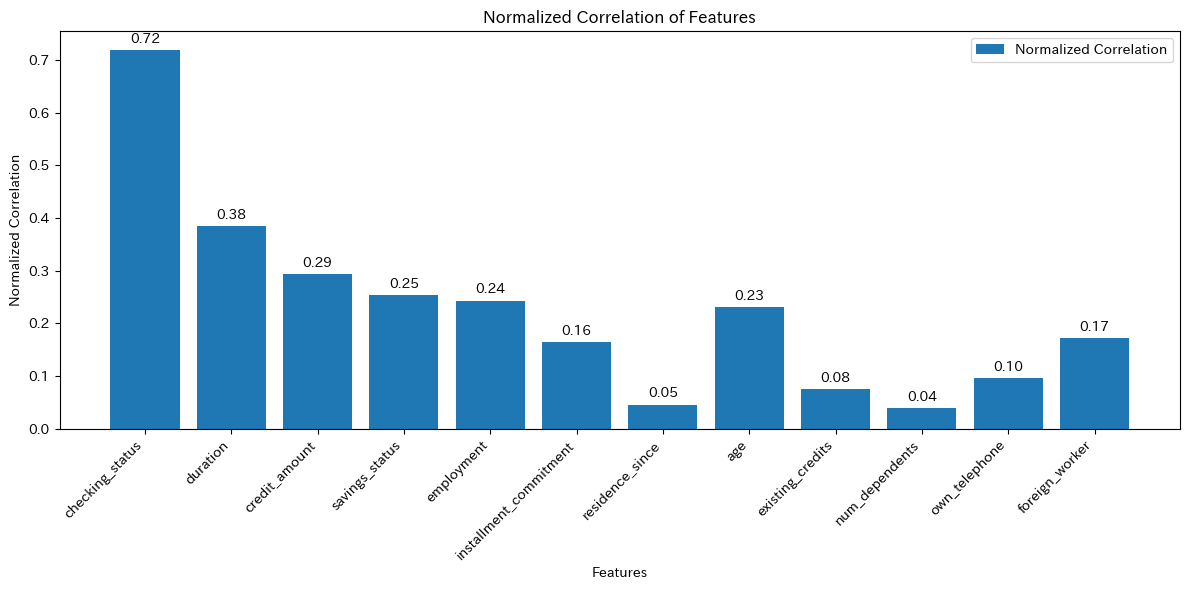
\includegraphics[width=0.8\textwidth]{images/従来手法_特徴量重要度.png}
%     \caption{従来手法:各特徴量における重要度}
%     \label{fig:default_method_feature_importance}
% \end{figure}


\subsection{従来手法の課題}

この手法について二つの問題をはらんでいる可能性がある

一つ目に特定の特徴量に対するノイズが集中してしまう可能性があることである.特徴量重要度の算出方法(式(6))において,相関係数に対して正規化処理を行っている.機械学習手法を利用する際に,特徴量ごとにとり得る範囲(スケール)が大きく異なることで過学習などの問題が発生してしまう可能性がある.正規化はこの問題を抑えるための手法として有用である.\cite{LawOfAwesomeDataScientist}相関係数の絶対値では0から1の範囲で特徴量の性質を表している.追加で正規化を行うと繊細な重要度を表現が難しくなる.特に重要度が極端に大きい特徴量に対してノイズを大きく避けるため,次に重要な特徴量へのノイズ集中してしまっている可能性をはらんでいる.よって元データの特徴を捉えた特徴量重要度の算出が重要になっている.

二つ目に,敵対的サンプルの出力が連続値であることが挙げられる.離散値を持つ特徴量に対して連続値を取ることで,現実的でない値をとってしまっている.このため,連続値の敵対的サンプルを離散値に変換する必要がある.


\section{提案手法}
\subsection{提案手法の概要}
前述の通り,従来手法では特定の特徴量に対する過剰なノイズが付与されている問題が存在する.また元データの特徴量が離散値であるにも限らず,連続値として敵対的サンプルが生成されている.この解決のため,特徴量に対する重要度算出法の改善と出力データの離散化を行う.
\subsection{重要度算出法の改善}
重要度算出法として,元データの重要度を維持しつつ,特定の特徴量の重要度が大きくなることを防ぐため,以下の式を提案する.

\autoequation{\bm{v}' = \|\rho_{\bm{X},Y}\|}
\autoequation{\bm{v}'' = \sqrt{\cfrac{\|\rho_{\bm{X},Y}\|}{\sum^{d}_{i=1}{(\|\rho_{\bm{X_i},Y}\|)^2}}}}

式(7)では,特徴量 $\bm{X}$ と目的変数 $\bm{Y}$ の相関係数の絶対値を用いる.これは従来手法で行っている重要度の算出から正規化の処理を外したものである.
式(8)では,従来手法の重要度算出法に平方根したものである.
従来手法では,各特徴量について相関係数の絶対値を正規化したものを使用していた.この算出法はデータの特性に合わせた重要度を算出することができている.しかし,今回のデータセットの場合前述の通り,一番重要度の高い特徴量と二番目以降に重要度の高い特徴量でさが大きく,一番を大きい特徴量に対して強いノイズの回避傾向がみて取れる.よって二番目に重要度の大きい特徴量に対して大きなノイズを加えてしまうような状態となっている.よってこれらの問題を解決するため,式(7)では正規化処理を外し,式(8)では平方根を導入した.相関係数というのは-1~1までの値である変数と変数の関係を表現したものである.よって正規化を行う必要はそこまでなく返って今回のような状態を引き起こしてしまう可能性がある.また,式(8)で平方根を導入した経緯として,小さい値ほど大きく,大きい値ほど小さくする特性がある.これにより,ノイズを強く回避する特徴を和らげることができ,より自然な敵対的サンプルを生成できる可能性がある.

\subsection{出力データの離散化手法}

先ほどの重要度特徴量算出により生成された敵対的サンプルは連続値であるため離散化の提案を行う.
一つ目に,小数部分の四捨五入による整数化である.この方法は,連続値を離散値に変換する際に最も一般的な方法であり,世間一般に広く使われている.しかし,四捨五入はその小数第一位,二位の値によって固定した変更が行われてしまい,情報損失の可能性がある.そこで二つ目にノイズが加わったノイズにランダム性を取り入れ,連続値を離散値に変換する方法を提案する.たとえば,ある特徴量が0である元データに対してノイズが加わり,0.4となった場合,四捨五入を行うと0に切り捨てられてしまいノイズが加わった効果を得ることができない.しかし,小数部分の数値を確率で見ることで40\%で繰り上げを行うことで,ノイズの損失を抑えることができる.よってこれらの2つの方法を実験で比較し,最適な離散化手法を提案する.

\section{実験}
\subsection{実験概要}
提案手法によるより自然な敵対的サンプルが生成可能なのかどうか有効性を検証するため,敵対的サンプルの生成実験を行った.前述の通り,提案手法に示した重要度算出法と離散化手法を組み合わせ,敵対的サンプルを生成する.さらに,得られた敵対的サンプルの具体的な値について,適切か否かの確認を行う.
\subsection{実験条件}
今回の実験は,銀行のローンの審査システムについての機械学習モデルを想定し,誤分類を引き起こす敵対的サンプルの生成を行うことを目的とした.パラメータの設定は従来研究\cite{ballet2019imperceptible}に準拠している.今回使用する機械学習モデルは,12個の特徴量を入力とし,2つのクラス(承認または拒否)を出力するニューラルネットワークである.このネットワークは,100個のノードを持つ隠れ層が6層にわたって配置された全結合型のモデルである.隠れ層はReLU関数で活性化され,出力層はバイナリクラス分類のためにSoftmax関数が使用されている.これらのモデルを図示したものを下に示す.

\begin{figure}[H]
    \centering
    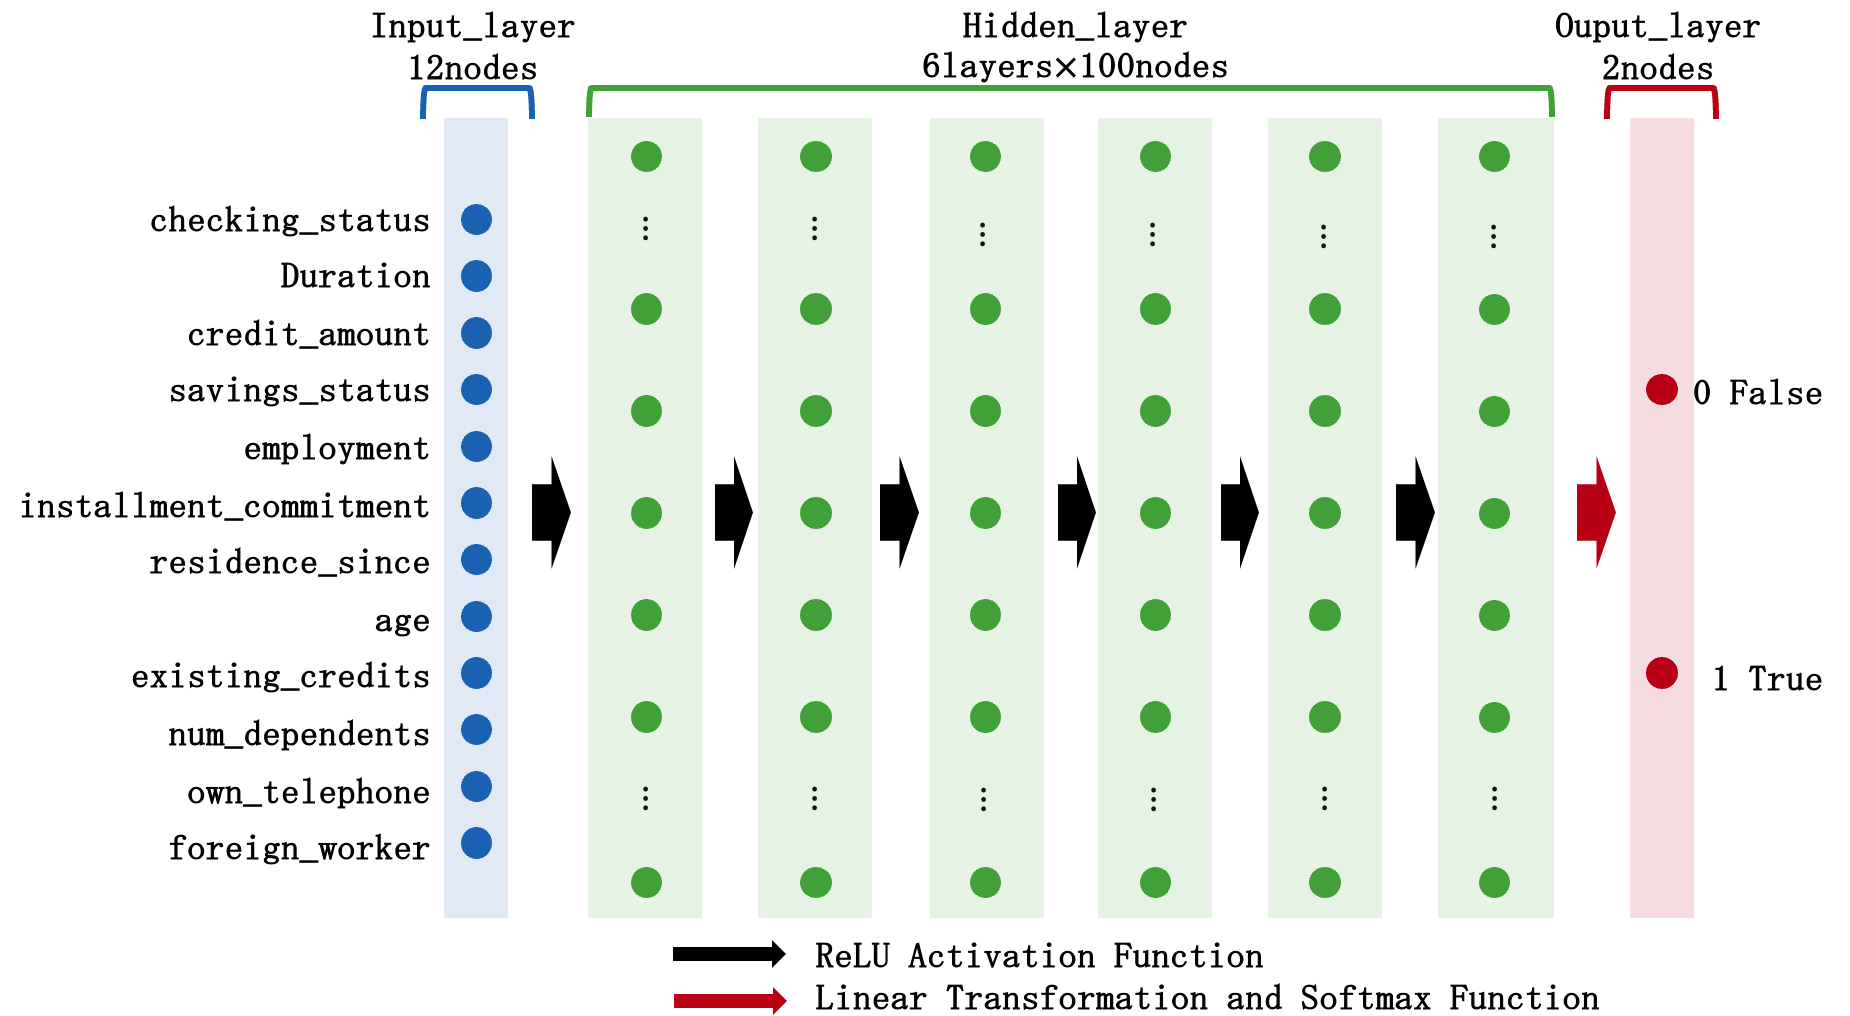
\includegraphics[width=0.8\textwidth]{images/審査モデル.png}
    \caption{銀行のローン審査を行う機械学習モデルの構造}
    \label{fig:adversarial_example}
\end{figure}

また,学習においてBCELoss(Binary Cross Entropy Loss)が損失関数として使用されている.モデルが各サンプルに対して予測した確率と実際のラベルとの誤差を計算し,二値分類における誤差を最小化する.最適化アルゴリズムにはAdamを使用し,学習率は $1.0 \times 10^{-4}$ に設定されている.バッチ学習を行い,バッチサイズは $N=100$ です.データを小分けにして学習を進め,予測精度はkeras.utils.to\_categoricalを用いてワンホットエンコーディングに変換し,各バッチで予測精度を計算した後,全データで平均を取っている.これによりモデルの分類精度を評価する.

使用データは前述のUCI Machine Learning RepositoryのGerman Credit Data Setを使用する.1000件のデータに対して正解データのバランスを保つようにデータをサンプリングする.取得した600件のデータのうち300件を学習データ,250件をテストデータ,残りを検証データに分割する.
まず,学習データでモデルの学習を行い,その後テストデータによるモデルの評価を行う.次にテストデータからランダムに10件取得し,それらをベースにノイズを加え敵対的サンプルを生成する.生成された敵対的サンプルに対して以下の評価指標を用いて評価を行う.

\subsection{評価指標}
提案手法の有効性の評価として以下の3つの指標を用い比較を行う.
一つ目に敵対的サンプルが元データと異なるクラスに分類されることを評価する指標である.これを成功率と呼び,式(9)に示す.
\autoequation{成功率 = \cfrac{|\hat{\mathbb{X}}|}{|\mathbb{X}|}}
ここで $\hat{\mathbb{X}}$ は生成された敵対的サンプルが元データと異なるクラスに分類されたサンプルの集合であり,$\mathbb{X}$ は全サンプルの集合である.この指標が大きいほど敵対的サンプルが元データと異なるクラスに分類されることが多いことを示す.

二つ目に敵対的サンプル生成前のサンプルと生成後のサンプル間の距離を評価する指標である.これを平均距離と呼び,式(10)に示す.
\autoequation{平均距離 = \cfrac{1}{N} \sum^{N}_{i=1} \sqrt{\sum^{d}_{j=1}(\mathrm{orig}_{i, j}-\mathrm{adv}_{i, j})^2}}
この指標が小さいほどノイズが小さく,元データに近いサンプルが生成されていることを示す.

三つ目に先ほどの平均距離に対して各特徴量の重要度で重み付けした指標である.これを重み距離と呼び,式(11)に示す.
\autoequation{重み距離 =  \cfrac{1}{N} \sum^{N}_{i=1} \sqrt{\sum^{d}_{j=1}( | \mathrm{orig}_{i, j}-\mathrm{adv}_{i, j}| \cdot v_i )^2}}
ここで使用する重要度 $\bm{v}$ は,従来手法で使用していた特徴量重要度 $\bm{v}$ と同様のものを使用する.この指標が小さいほど分類に対する重要度の高い特徴量に対するノイズが小さいことを示す.

各指標を組み合わせて使用することで,生成した敵対的サンプルの「有効性」と「自然さ」の両面を総合的に評価することを目指す.

\subsection{実験結果}
まず成功率について確認する.
\begin{table}[H]
    \centering
    \caption{実験結果:成功率}
    \begin{tabular}{|c|c|c|c|} \hline
        離散化 & 従来手法(式(6)) & 重要度算出(式(7)) & 重要度算出(式(8)) \\ \hline
        なし & 1.0 & 1.0 & 1.0 \\ \hline
        離散化(四捨五入) & 1.0 & 1.0 & 1.0 \\ \hline
        離散化(ランダム) & 1.0 & 1.0 & 1.0 \\ \hline
    \end{tabular}
\end{table}
すべての手法で10個の敵対的サンプルの生成ができた.

次に平均距離について確認する.
\begin{table}[H]
    \centering
    \caption{実験結果:平均距離}
    \begin{tabular}{|c|c|c|c|} \hline
        離散化 & 従来手法(式(6)) & 重要度算出(式(7)) & 重要度算出(式(8)) \\ \hline
        なし & 0.377 & 0.260 & 0.173 \\ \hline
        離散化(四捨五入) & 0.399 & 0.264 & 0.163 \\ \hline
        離散化(ランダム) & 0.454 & 0.347 & 0.233 \\ \hline
    \end{tabular}
\end{table}
この結果から,従来手法よりも提案手法は,元データに近い敵対的サンプルを生成できていることがわかる.離散化手法については四捨五入の方がよりノイズが小さくなっていることがわかる.重要度については式(8)が一番小さい距離を示しており,四捨五入による離散化手法では,この実験で最小の距離を示す.

次に重み距離について確認する.
\begin{table}[H]
    \centering
    \caption{実験結果:重み距離}
    \begin{tabular}{|c|c|c|c|} \hline
        離散化 & 従来手法(式(6)) & 重要度算出(式(7)) & 重要度算出(式(8)) \\ \hline
        なし & 0.043 & 0.060 & 0.173\\ \hline
        離散化(四捨五入) & 0.044 & 0.048 & 0.061 \\ \hline
        離散化(ランダム) & 0.051 & 0.105 & 0.105 \\ \hline
    \end{tabular}
\end{table}
この結果から,提案手法は従来手法よりも良いスコアを出すことができなかった.しかし,重要度算出(式(7))における四捨五入による離散化手法では,一番従来手法に近い距離を示している.

最後に,従来手法(式(6)),提案手法(式(7)),提案手法(式(8))における特徴量重要度について以下の図に示す.
\begin{figure}[H]
    \centering
    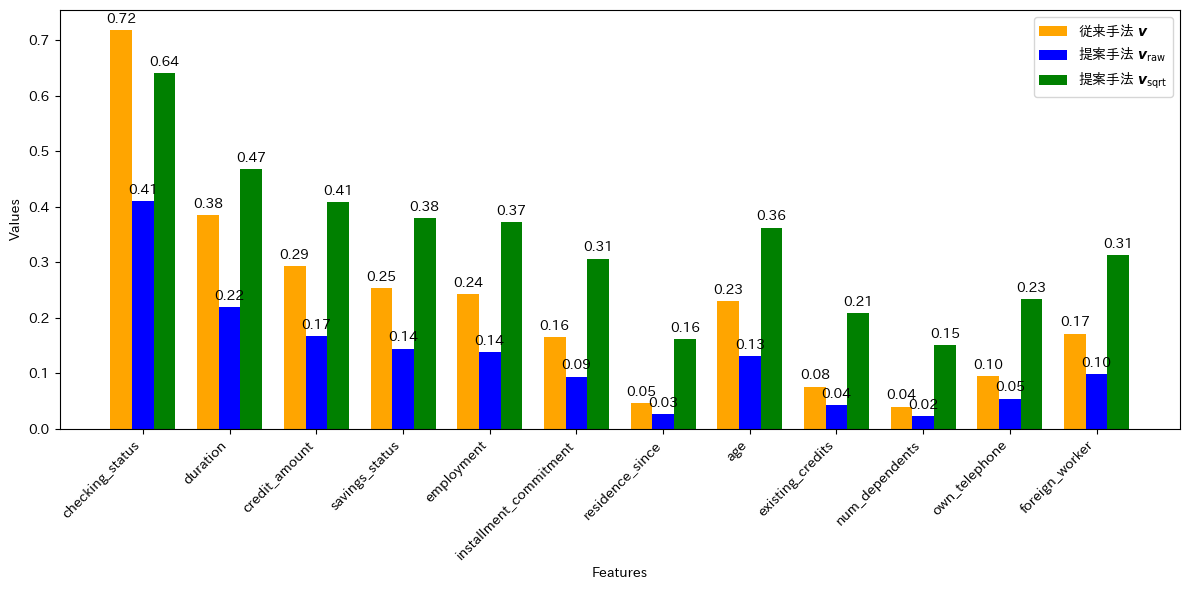
\includegraphics[width=0.8\textwidth]{images/実験_重要度算出の結果.png}
    \caption{実験結果:各特徴量における重要度}
    \label{fig:adversarial_example}
\end{figure}
重要度について比較すると,従来手法では,checking\_statusに対する重要度が飛び抜けており,次に重要度の高い特徴量との差が大きいことが指摘されていた.提案手法ではその差が小さくなっていることが確認できる.また,提案手法(式(8))では,特徴量の重要度がより均等になっていることがわかる.これにより,提案手法はより自然な敵対的サンプルを生成できることが示された.
\subsection{考察}
以上の実験結果を考察すると,提案手法は従来手法よりも元データに近い敵対的サンプルを生成することが示された.特に成功率および平均距離の指標では,提案手法(式(7))が従来手法を上回る性能を発揮した.この結果は,提案手法が重要度算出と離散化の適切な組み合わせにより,必要最小限のノイズで誤分類を誘発する敵対的サンプルを生成できたためと考えられる.一方で,重み距離の結果において提案手法(式(8))が劣る原因としては,重要度算出アルゴリズムにおける平方根操作の影響が挙げられる.平方根は大きい値を小さく小さい値を大きくするため図8で従来手法と比較するとより滑らかな重要度
となっている.分類性能に影響を与える重要な特徴量に対する変化が抑制されなかったことが考えられる.これにより自然な敵対的サンプルの生成を行うことができなかったということがわかる.

さらに,評価結果に基づき元データ,従来手法,提案手法(式(7))による敵対的サンプルを比較した結果,提案手法によるサンプルはより「自然」であり,実運用環境における敵対的サンプル対策として有効であることが確認された.

\begin{table}[H]
    \centering
    \caption{元データと敵対的サンプルの比較}
    \begin{tabular}{|c|c|c|c|} \hline
        特徴量 & 元データ & 従来手法 & 提案手法 \\ \hline
        checking\_status & 0 & 0.09115 & 0\\ \hline
        duration & 14 & 8.89098 & 15 \\ \hline
        credit\_amount & 8978 & 7153.84454 & 9169 \\ \hline
        savings\_status & 0 & 0.083762 & 0\\ \hline
        employment & 4 & 3.947638  & 4 \\ \hline
        installment\_commitment & 1 & 1.071917 & 1\\ \hline
        residence\_since & 4 & 4.000000 & 2 \\ \hline
        age & 45 & 44.413271 & 45 \\ \hline
        existing\_credits & 1 & 1.000000 & 1 \\ \hline
        num\_dependents & 1 & 1.000000 & 1 \\ \hline
        own\_telephone & 1 & 0.992310 & 1 \\ \hline
        foreign\_worker & 1 & 1.000000 & 1 \\ \hline
    \end{tabular}
\end{table}

実際のデータについても,離散化により自然な敵対的サンプルになっていることがわかる.また,ノイズの大きさについてもchecking\_statusのノイズを避けるあまり,durationやcredit\_amountに対してノイズが大きくなっている従来手法に対して,提案手法は小さくすることができている.これにより,提案手法はより自然な敵対的サンプルを生成できることが示された.

\section{考察}
% \subsection{考察}
以上の実験結果をまとめると,提案手法は従来手法よりも元データに近い敵対的サンプルを生成することが示された.

特に成功率および平均距離の指標では,提案手法( $\bm{v}_{\mathrm{raw}}$ )が従来手法を上回る性能を発揮した.図8や実際のデータから示されるように,従来手法では重要度の大きい特徴量に対するノイズの回避傾向から次点の重要度の高い特徴量に対するノイズが大きくなってしまっていたことが言える.提案手法はこれらのノイズが抑制され,ノイズの平均距離を小さく,重み距離を同程度にまですることができた.この結果は,提案手法が重要度算出と離散化の適切な組み合わせにより,必要最小限のノイズで誤分類を誘発する敵対的サンプルを生成できたためと考えられる.

一方で,重み距離の結果において提案手法( $\bm{v}_{\mathrm{sqrt}}$ )が劣る原因としては,重要度算出アルゴリズムにおける平方根操作の影響が挙げられる.平方根は大きい値を小さくするため図8で従来手法と比較するとより滑らかな重要度となっている.分類性能に影響を与える重要な特徴量に対する変化が抑制されなかったことが考えられる.これにより自然な敵対的サンプルの生成を行うことができなかったということがわかる.

さらに,評価結果に基づき元データ,従来手法,提案手法(式(7))による敵対的サンプルを比較した結果,提案手法によるサンプルはより人間に知覚することが難しく,元のデータ分布に近い実運用環境における敵対的サンプル対策として有効であることが確認された.

\section{結論}
\subsection{まとめ}
本研究では,入力データの特徴とその重要度を考慮した敵対的サンプル生成手法について提案を行った.従来手法は,表形式データに対するノイズの付加を行う画期的な手法であったが,特定の特徴量に対して過剰なノイズが付与される問題が存在し,離散値を持つ表形式データに対して連続値の敵対的サンプルが生成される問題があった.これらの問題に対処するため,本研究では特徴量の重要度算出方法を改善し,出力データの離散化を行うことで,より自然な敵対的サンプルの生成を実現した.

具体的には,従来手法で用いられていた相関係数の正規化処理を見直し,重要度算出方法を改善することで,特定の特徴量に対する過剰なノイズの付与を抑制した.また,出力データの離散化手法として四捨五入およびランダム離散化を導入し,元データの特性を保持しつつ,現実的な敵対的サンプルを生成することができた.

実験結果から,提案手法は従来手法に比べて,元データに対する変更が少なく,より自然な敵対的サンプルを生成できることが示された.特に,重要度算出法( $\bm{v}_{\mathrm{sqrt}}$ )と四捨五入による離散化手法の組み合わせが最も効果的であり,元データの特徴を保持しつつ,適切なノイズを付加することで,より自然な敵対的サンプルを生成することができた.

さらに,提案手法は従来手法に比べて,成功率および平均距離の指標で優れた性能を示した.これにより,提案手法が従来手法に比べて,より効果的に敵対的サンプルを生成できることが確認された.一方で,重み距離の指標においては,提案手法( $\bm{v}_{\mathrm{sqrt}}$ )が劣る結果となったが,これは重要度算出アルゴリズムにおける平方根操作の影響によるものであると考えられる.

本研究の成果は,機械学習モデルの堅牢性を向上させるための敵対的学習の重要な礎となるより精度の高い敵対的サンプルの生成を行うことができた,今後の研究においても,提案手法をさらに改良し,より広範なデータセットやモデルに適用することで,その有効性を検証していくことが期待される.また,提案手法を実運用環境に適用することで,機械学習モデルの安全性を向上させ,敵対的サンプルによる攻撃からシステムを保護することが可能となる.

\subsection{今後の課題}
本研究では,使用したデータセットのみに適用を行った.実験結果として他のデータセットに対しても提案手法を適用することで,汎用性の高い手法であるかを検証する必要がある.また,提案手法のハイパーパラメータの調整や,他の敵対的サンプル生成手法との比較を行うことで,提案手法の有効性を評価する必要がある.さらに,今回の実験の中で生成された敵対的サンプルについてデータによっては評価が良くない場合もあったが,異なるデータセットにおいて良い評価を得ることができたことから,複数の敵対的サンプル生成手法を組み合わせるアンサンブル学習などが効果的である可能性がある.この点についても今後の研究で調査を行うべきである.


% 謝辞
\acknowledgements
% 謝辞の文面は過去の(豊田高専を含む)謝辞や,藤原の博士論文を参考にしてください.
% 博士論文の謝辞は長大ですが,卒業研究論文の謝辞をそんなに長くする必要は全くないと思います.
本論文の執筆にあたり,多くの方々から多大なるご支援とご指導を賜りましたことを,心より感謝申し上げます.
まず,指導教員の東京都市大学メディア情報学部情報システム学科 三川健太准教授には研究の最終段階に至るまで,度重なるご指導,ご鞭撻を賜りましたことを深く感謝いたします.
また,東京都市大学大学院環境情報学研究科環境情報学専攻 福田竜也氏には,研究の進行において多くの有益なアドバイスをいただきました.福田氏のご助言により研究をより前に進めることができました.心から感謝いたします.
さらに,日々のゼミ活動において多くの助言を賜りました,三川研究室の皆様にも感謝いたします.特に研究の環境構築において多大なるご協力をいただいた同研究室の佐竹航希さんに,心より感謝いたします.
皆様のご支援とご指導に,改めて感謝の意を表します.

% 参考文献
% BibTeX を使って参考文献のリストをつくって下さい.
% proceedings.bib: 雑誌名や国際会議の名称をマクロ化しています
% ref.bib: ここに参考文献を書くと良いと思います.元々博士論文に使った論文の情報が載っています.
% ref.bib以外のファイルに分けることも可能です.単純にカンマで区切ってファイル名(.bib除く)を
% \bibliographyの引数に追加してください.
\bibliography{proceedings,ref}

% 付録
% 付録には,本文に直接載せるべきではない,文字通り付録となる要素を載せます.
% 例えば,詳細な数式の展開であったり,アンケートや実験の詳細な(ほぼ完全な)結果だったりを載せます.
% 必要であれば以下の3行のコメントアウトを外して付録を加えてください.
\appendix
% サンプルです.全部削除してください.


\end{document}

